\chapter{Triangle Theorems and Formulas}
\begin{figure}[H]
		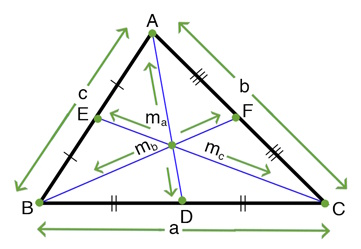
\includegraphics[scale=1, center]{./image/Triangle-Formula.jpg}
\end{figure}
\section*{1. Basic Angle Rules}
\begin{align*}
A + B + C &= 180^\circ \\
\text{Exterior Angle} &= \text{Sum of two opposite interior angles}
\end{align*}

\section*{2. Side and Angle Relationships}
\subsection*{Law of Sines}
\[
\frac{a}{\sin A} = \frac{b}{\sin B} = \frac{c}{\sin C}
\]

\subsection*{Law of Cosines}
\begin{align*}
c^2 &= a^2 + b^2 - 2ab\cos C \\
a^2 &= b^2 + c^2 - 2bc\cos A \\
b^2 &= a^2 + c^2 - 2ac\cos B
\end{align*}

\subsection*{Law of Tangents}
\[
\frac{a - b}{a + b} = \frac{\tan\left(\frac{A - B}{2}\right)}{\tan\left(\frac{A + B}{2}\right)}
\]

\section*{3. Area Formulas}
\subsection*{Basic}
\[
\text{Area} = \frac{1}{2} \cdot \text{base} \cdot \text{height}
\]

\subsection*{Heron’s Formula}
Let \( s = \frac{a + b + c}{2} \):
\[
\text{Area} = \sqrt{s(s - a)(s - b)(s - c)}
\]

\subsection*{Using Sine}
\[
\text{Area} = \frac{1}{2} ab \sin C
\]

\section*{4. Right Triangle Formulas}
\subsection*{Pythagorean Theorem}
\[
a^2 + b^2 = c^2
\]

\subsection*{Trigonometric Ratios}
\begin{align*}
\sin \theta &= \frac{\text{opposite}}{\text{hypotenuse}} \\
\cos \theta &= \frac{\text{adjacent}}{\text{hypotenuse}} \\
\tan \theta &= \frac{\text{opposite}}{\text{adjacent}}
\end{align*}

\section*{5. Medians (Mid-Height)}
\begin{align*}
m_a &= \frac{1}{2} \sqrt{2b^2 + 2c^2 - a^2} \\
m_b &= \frac{1}{2} \sqrt{2a^2 + 2c^2 - b^2} \\
m_c &= \frac{1}{2} \sqrt{2a^2 + 2b^2 - c^2}
\end{align*}

\section*{6. Heights (Altitudes)}
\begin{align*}
h_a &= \frac{2 \cdot \text{Area}}{a} \\
h_b &= \frac{2 \cdot \text{Area}}{b} \\
h_c &= \frac{2 \cdot \text{Area}}{c}
\end{align*}

\section*{7. Equilateral Triangle (side = \(a\))}
\begin{align*}
\text{Each angle} &= 60^\circ \\
\text{Height} \ h &= \frac{\sqrt{3}}{2} a \\
\text{Area} &= \frac{\sqrt{3}}{4} a^2
\end{align*}

\section*{8. Coordinate Geometry}
\subsection*{Distance between points}
\[
d = \sqrt{(x_2 - x_1)^2 + (y_2 - y_1)^2}
\]

\subsection*{Area from coordinates}
\[
\text{Area} = \frac{1}{2} \left| x_1(y_2 - y_3) + x_2(y_3 - y_1) + x_3(y_1 - y_2) \right|
\]

\subsection*{Centroid}
\[
G = \left( \frac{x_1 + x_2 + x_3}{3}, \frac{y_1 + y_2 + y_3}{3} \right)
\]

\section*{9. Inradius and Circumradius}
\subsection*{Inradius}
\[
r = \frac{\text{Area}}{s} = \sqrt{\frac{(s-a)(s-b)(s-c)}{s}}
\]

\subsection*{Circumradius}
\[
R = \frac{abc}{4 \cdot \text{Area}} = \frac{a}{2 \sin A}
\]
